\documentclass[11pt]{article}
\usepackage[margin=1in]{geometry}
\usepackage[utf8]{inputenc}
\usepackage[T1]{fontenc}
\usepackage{lmodern}
\usepackage{amsmath,amssymb}
\usepackage{graphicx}
\usepackage{booktabs}
\usepackage{xcolor}
\usepackage[colorlinks=true,linkcolor=blue!60!black,citecolor=blue!60!black,urlcolor=blue!60!black]{hyperref}
\usepackage[numbers,sort&compress]{natbib}

\title{Where Small Quantum Classifiers Help, and Where They Don't:\\
Fair Baselines and Real-Hardware Results on IBM Heron}
\author{Vivek Reddy\\\small Independent researcher}
\date{November 2026}

\begin{document}
\maketitle

\begin{abstract}
We compare small quantum neural networks (QNNs) with classical models under a fixed protocol: classical baselines receive the same inputs and are tuned by cross-validation, a strong classical reference is always reported, hardware runs are compared with noise-free simulation on identical inputs, and hardware deviations are tested against the exact shot-noise expectation.
On two text tasks, a 4-qubit QNN fed by a sentence encoder is within 1.5 percentage points of tuned classical models on the same four features: slightly but significantly below on sentiment (0.757 $\pm$ 0.007 vs.\ 0.772 over three seeds) and statistically tied on CVE severity (0.699 $\pm$ 0.015 vs.\ 0.691).
A controlled ablation attributes most of the effect of circuit design to the data encoding (21 points), while 2--6 qubits changed accuracy by at most 1.2 points.
On IBM's \texttt{ibm\_marrakesh}, with 200 inputs per task and repeated runs on fixed physical qubits, device accuracy is statistically indistinguishable from noise-free simulation, but the device shows a small, resolvable bias in output probability ($-0.006$ and $-0.004$, 95\% CIs excluding zero).
A noise model of the same device reproduces this bias; a model of an older 5-qubit device overstates it about fivefold.
In exact simulation of quantum data, a learned two-copy QNN distinguishes pure from mixed states with 16--64 copies per seed from 2 to 6 qubits, while the classical-shadow method we test needs 128--4{,}096, a small-scale illustration of a known multi-copy separation.
All code, data pipelines, result files and job identifiers are public.
\end{abstract}

\section{Introduction}
Claims of quantum advantage in machine learning are hard to evaluate when results are reported without matched classical baselines~\cite{bowles2024better}.
We ask a narrow question: for small, trainable quantum classifiers that run on current hardware, on which tasks do they differ from well-tuned classical models, and how much does real-device noise change their outputs?

We report two projects. The first trains a 4-qubit QNN on classical data, including two text-classification tasks, and runs the trained circuits on IBM Quantum hardware. The second classifies quantum states directly, a setting where theory predicts separations for learners with quantum memory~\cite{huang2022experiments,chen2021memory,aharonov2022qam}; its main purity result is in exact simulation only. Our contributions are:
\begin{itemize}
  \item an evaluation protocol that keeps quantum and classical models on identical inputs, tunes the classical baselines, and compares hardware with simulation on identical inputs (Section~\ref{sec:protocol});
  \item evidence, with seed variation and paired confidence intervals, that a well-designed QNN is close to but not better than tuned classical models on the same features for two text tasks, and a controlled ablation of the circuit design (Section~\ref{sec:classical});
  \item a repeated hardware study on fixed physical qubits showing statistically indistinguishable accuracy but a small resolvable output bias, reproduced by a noise model of the same device (Section~\ref{sec:hardware});
  \item a small-scale simulation of the copy-complexity gap between a learned two-copy QNN and a classical-shadow baseline for purity testing, with per-seed results (Section~\ref{sec:quantum}).
\end{itemize}

\section{Evaluation protocol}\label{sec:protocol}
\begin{enumerate}
  \item \textbf{Same inputs.} Classical baselines (logistic regression and an RBF SVM; an MLP where noted) receive exactly the features encoded into the circuit.
  \item \textbf{Tuned baselines and a classical reference.} Same-feature baselines are tuned by 5-fold cross-validation on the training data only. We also report logistic regression on the full feature set and all training data.
  \item \textbf{Same inputs on hardware.} Device runs use a fixed random subset of the test set; they are compared only with the noise-free simulator on that subset.
  \item \textbf{Shot noise as the null hypothesis.} Prediction changes on hardware are compared with the exact distribution expected from finite sampling alone, and repeated in independent jobs.
\end{enumerate}
\paragraph{Disclosure.} The circuit design and feature-reduction method were chosen in exploratory runs that reported test-set accuracy; no separate validation set was held out for those choices. The ablation in Section~\ref{sec:classical} and the multi-seed results quantify how sensitive the conclusions are to them. Rule 3 was introduced after our first hardware chart placed 40-input device accuracy beside 200-input simulator accuracy, which made the device appear better than the simulator on one dataset.

\section{Quantum classifiers on classical data}\label{sec:classical}
\paragraph{Model.} Inputs are reduced to one feature per qubit and min--max scaled to $[0,\pi]$ using the training data. The circuit repeats, twice, an $R_Y(x_i)$ encoding layer followed by one trainable \texttt{RealAmplitudes} layer (data re-uploading~\cite{perezsalinas2020reuploading,schuld2021encoding}); the class is the measured value of qubit~0 (class~1 if $P(1) > 0.5$). Weights are initialised uniformly in $[-\pi,\pi]$ from the seed and trained with L-BFGS-B (at most 60 iterations, one start) on the cross-entropy of the exact simulated output probabilities, with one-hot labels. We used Qiskit~1.4~\cite{qiskit} and qiskit-machine-learning~0.8.

\paragraph{Text data and partitions.} Texts are embedded with all-MiniLM-L6-v2~\cite{reimers2019sbert} (384 dimensions) and reduced to four features with partial least squares (PLS), fitted on the full training split; the scalers are also fitted on training data only.
\emph{Sentiment}: Rotten Tomatoes sentence polarity~\cite{pang2005seeing}, the standard 8{,}530/1{,}066 train/test split (the 1{,}066-sentence validation split is unused), balanced.
\emph{CVE severity}: 12{,}116 NVD descriptions with CVSS v3.1 scores, published 1~January--29~April 2024, labelled high/critical if the base score is at least 7.0, and split by publication date: training up to 9~April 2024 (9{,}692; 49.9\% high/critical), test after it (2{,}424; 42.2\%). The label shift explains the 0.578 majority-class baseline.
For each seed, the QNN and the same-feature baselines are trained on the same balanced random subset of 600 training texts; the full-embedding reference uses all training texts.

\begin{table}[h]
\centering
\small
\resizebox{\linewidth}{!}{%
\begin{tabular}{lcc}
\toprule
Model (test accuracy, mean $\pm$ std over 3 seeds) & Sentiment (1{,}066) & CVE severity (2{,}424) \\
\midrule
Majority class & 0.500 & 0.578 \\
QNN, 4 qubits & 0.757 $\pm$ 0.007 & 0.699 $\pm$ 0.015 \\
Logistic regression, same 4 features, defaults & 0.770 $\pm$ 0.000 & 0.688 $\pm$ 0.004 \\
Logistic regression, same 4 features, CV-tuned & 0.772 $\pm$ 0.002 & 0.689 $\pm$ 0.004 \\
RBF SVM, same 4 features, CV-tuned & 0.770 $\pm$ 0.004 & 0.691 $\pm$ 0.008 \\
Logistic regression, full embedding, all data (defaults / CV-tuned) & 0.774 / 0.774 & 0.715 / 0.702 \\
\midrule
Paired 95\% CI, QNN $-$ tuned logistic regression (seed 0) & [$-0.030$, $-0.002$] & [$-0.009$, $+0.023$] \\
\bottomrule
\end{tabular}}
\caption{Text tasks. Confidence intervals are percentile bootstraps over test items (2{,}000 resamples). Tuning grids: $C \in \{0.01,\dots,100\}$; for the SVM also $\gamma \in \{\text{scale}, 0.1, 1, 10\}$.}
\label{tab:text}
\end{table}

On sentiment the QNN is consistently about 1.5 points below the tuned classical models, and the paired interval excludes zero. On CVE severity the QNN is nominally ahead but the paired interval includes zero, so we read it as a tie. Cross-validated tuning of the full-embedding model lowered its CVE test accuracy (0.715 to 0.702), consistent with the label shift between the time-ordered splits.

\paragraph{Which design choice mattered?} An earlier design, using the \texttt{ZZFeatureMap} encoding~\cite{havlicek2019supervised}, parity readout of all qubits and training on 1{,}024-shot sampled probabilities with COBYLA, scored about 0.69 on breast cancer. Table~\ref{tab:ablation} changes one factor at a time from the final design, over three seeds (the seed sets the 70/30 split and the initial weights). The encoding accounts for most of the difference; the other choices, including the number of qubits between 2 and 6, change accuracy by at most 2.3 points.

\begin{table}[h]
\centering
\small
\resizebox{\linewidth}{!}{%
\begin{tabular}{lcc}
\toprule
Variant (breast cancer, 300 training / 171 test, PCA features) & Accuracy & vs.\ final \\
\midrule
Final: angle encoding, re-uploaded twice, qubit-0 readout, exact, L-BFGS-B, 4 qubits & 0.910 $\pm$ 0.011 & -- \\
\texttt{ZZFeatureMap} encoding (no re-upload), rest as final & 0.700 $\pm$ 0.032 & $-0.211$ \\
No re-uploading & 0.887 $\pm$ 0.015 & $-0.023$ \\
Parity readout & 0.924 $\pm$ 0.005 & $+0.014$ \\
COBYLA instead of L-BFGS-B & 0.903 $\pm$ 0.003 & $-0.008$ \\
Sampled (1{,}024-shot) training, COBYLA & 0.899 $\pm$ 0.012 & $-0.012$ \\
Original design (all of the above changes) & 0.690 $\pm$ 0.051 & $-0.220$ \\
2 qubits / 6 qubits & 0.916 / 0.899 & $+0.006$ / $-0.012$ \\
\bottomrule
\end{tabular}}
\caption{One-factor ablation, mean $\pm$ std over 3 seeds; all variants are evaluated with exact probabilities. This is a single dataset and should be read as indicative.}
\label{tab:ablation}
\end{table}

Figure~\ref{fig:bench} gives the same comparison on three standard datasets and on the two text tasks, using smaller, separate splits (300 training and at most 200 test items, PCA for the tabular data). The QNN is within 0--10 points of the best classical model on each and above logistic regression only on the nonlinear two-moons task, where the RBF SVM is best. The text-task numbers in Table~\ref{tab:text} supersede the text-task bars in this figure.

\begin{figure}[h]
\centering
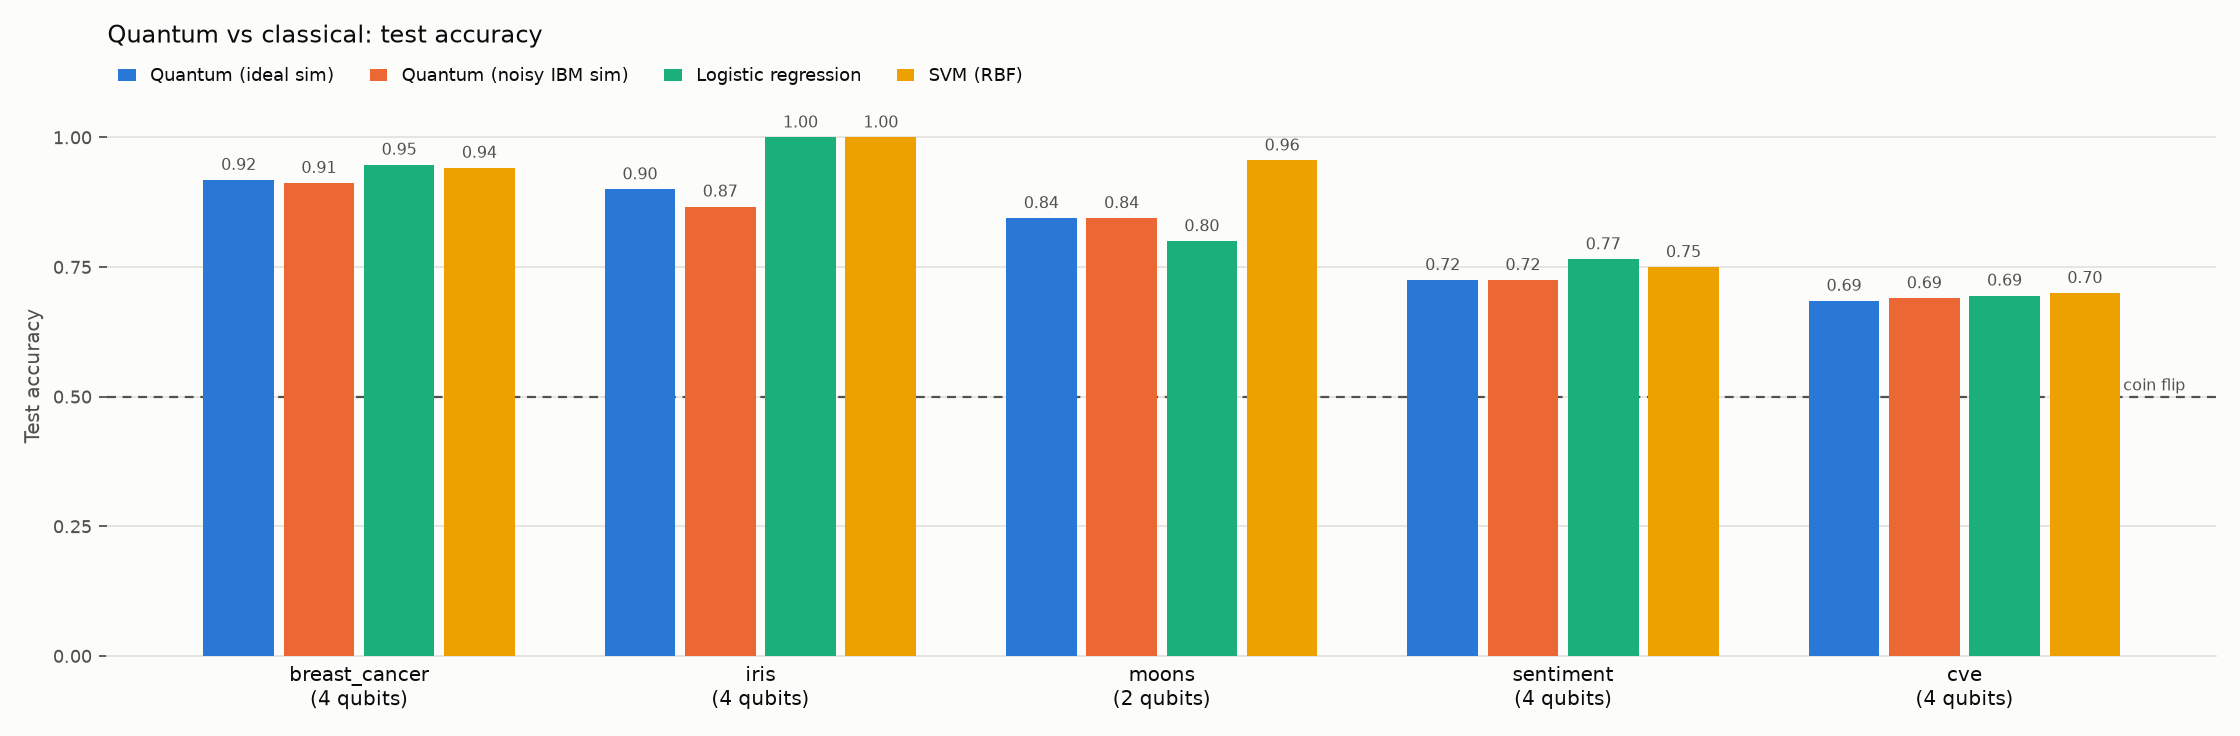
\includegraphics[width=\linewidth]{figures/agi_benchmark.png}
\caption{Benchmark on smaller, separate splits: test accuracy of the QNN (noise-free and with the \texttt{FakeManilaV2} noise model) and classical models on identical reduced features, one seed.}
\label{fig:bench}
\end{figure}

\section{Real-hardware behaviour}\label{sec:hardware}
\paragraph{Setup.} We ran the trained sentiment and CVE models (seed 0, Table~\ref{tab:text}) on IBM's 156-qubit Heron device \texttt{ibm\_marrakesh} through the free Open Plan, with \texttt{SamplerV2}, 1{,}024 shots and no error mitigation or dynamical decoupling. Each circuit was transpiled once with Qiskit's preset pass manager (optimisation level 1, \texttt{seed\_transpiler}=0), so every run used the same physical qubits (0--3); the compiled circuit has depth 37 with six CZ gates. At execution time the readout errors of these qubits were 0.006--0.024 and the CZ errors 0.0022--0.0027 (full snapshot and job identifiers in Appendix~\ref{app:repro}). For each task we drew a fixed, stratified random sample of 200 test inputs and ran it as separate jobs: three for CVE severity, one in a later session, and one for sentiment.

\paragraph{Statistics.} For an input with noise-free probability $p$ and $N$ shots, the probability that sampling alone changes the prediction is the exact binomial tail
\begin{equation}
q(p) = \begin{cases} P(K \le N/2), & p > 1/2,\\ P(K > N/2), & p \le 1/2,\end{cases}\qquad K \sim \mathrm{Bin}(N, p).
\end{equation}
Treating inputs and runs as independent, the total number of changed predictions follows a Poisson-binomial distribution, which we compute exactly by convolution. Bias is the mean signed difference between device and noise-free $P(\text{class }1)$, with a 95\% bootstrap interval over inputs.

\begin{figure}[h]
\centering
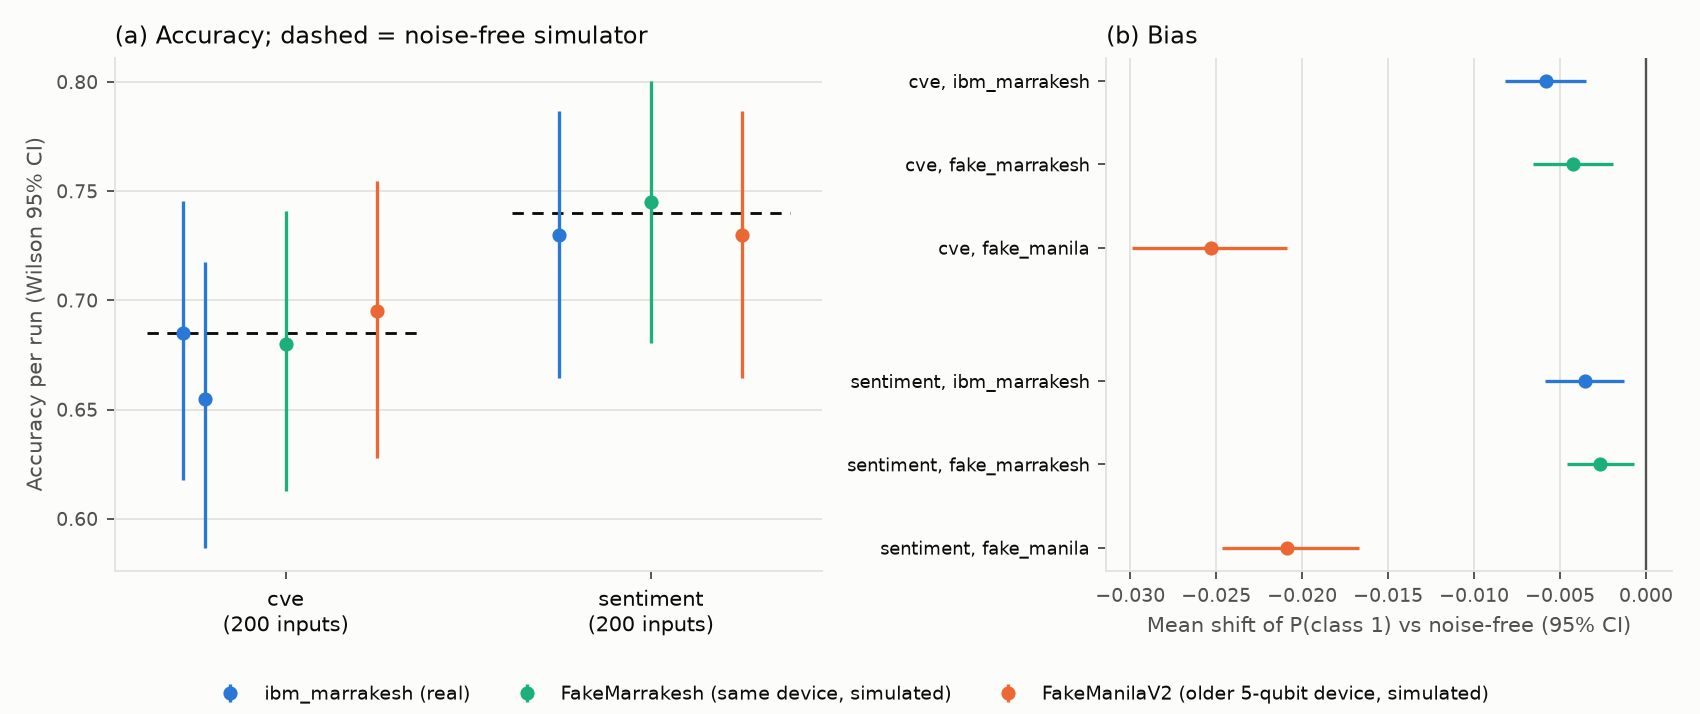
\includegraphics[width=\linewidth]{figures/agi_hardware_study.png}
\caption{Hardware study, 200 inputs per task. (a) Accuracy per run with Wilson 95\% intervals; dashed lines are noise-free accuracy on the same inputs. (b) Mean signed shift of $P(\text{class }1)$ relative to noise-free simulation, pooled over runs, with 95\% bootstrap intervals.}
\label{fig:hw}
\end{figure}

\paragraph{Results.} Figure~\ref{fig:hw} and Table~\ref{tab:hw} summarise the study. Device accuracy is statistically indistinguishable from noise-free accuracy: with 200 inputs, Wilson intervals span about $\pm 0.065$, and the numbers of changed predictions are consistent with shot noise ($p = 0.15$ for CVE over two runs, $0.37$ for sentiment). Repeated runs agree on 96\% of predictions. The device nevertheless shows a small, statistically resolvable bias towards class~0 on both tasks, of $-0.006$ and $-0.004$ in probability, with intervals that exclude zero. Such a bias can change predictions for inputs near the decision boundary, so label agreement alone understates the effect of noise.

\begin{table}[h]
\centering
\small
\resizebox{\linewidth}{!}{%
\begin{tabular}{llcccc}
\toprule
Task & Backend & Accuracy per run & Changed / expected & $p$ & Bias [95\% CI] \\
\midrule
CVE (ideal 0.685) & \texttt{ibm\_marrakesh} & 0.685, 0.655 & 12 / 8.9 & 0.15 & $-0.0058$ [$-0.0082$, $-0.0035$] \\
 & FakeMarrakesh & 0.680 & 3 / 4.4 & 0.86 & $-0.0043$ [$-0.0066$, $-0.0019$] \\
 & FakeManilaV2 & 0.695 & 12 / 4.4 & $<0.001$ & $-0.0253$ [$-0.0299$, $-0.0209$] \\
Sentiment (ideal 0.740) & \texttt{ibm\_marrakesh} & 0.730 & 4 / 3.1 & 0.37 & $-0.0035$ [$-0.0059$, $-0.0013$] \\
 & FakeMarrakesh & 0.745 & 3 / 3.1 & 0.63 & $-0.0027$ [$-0.0046$, $-0.0007$] \\
 & FakeManilaV2 & 0.730 & 8 / 3.1 & 0.003 & $-0.0209$ [$-0.0246$, $-0.0167$] \\
\bottomrule
\end{tabular}}
\caption{Hardware study, 200 inputs per task, 1{,}024 shots. ``Changed / expected'' counts predictions that differ from the noise-free prediction, against the exact shot-noise expectation; $p = P(\text{total} \ge \text{observed})$ under shot noise alone.}
\label{tab:hw}
\end{table}

\paragraph{Noise models.} \texttt{FakeMarrakesh}, Qiskit's noise model built from a calibration snapshot of the same device, reproduces both the accuracy behaviour and the bias of the real device within the intervals. \texttt{FakeManilaV2}, a model of an older 5-qubit device, overstates the bias about fivefold and changes significantly more predictions than shot noise allows. This compares two specific noise models on one circuit; it suggests matching the noise model to the device, rather than a general statement about noise models.

\paragraph{Earlier, smaller run.} A first run on 40 inputs per dataset (30 for iris) on the previous day reproduced the noise-free predictions on four of five datasets; CVE changed three predictions, and three repeats on the same 40 inputs gave 5 changes against 3.45 expected (exact $p = 0.24$; 8 against 4.6, $p = 0.063$, including the first run). These smaller samples motivated the study above.

\section{Quantum classifiers on quantum data}\label{sec:quantum}
The second project gives models direct access to quantum states in exact simulation; classical learners (logistic regression, RBF SVM, MLP) receive classical-shadow estimates~\cite{huang2020shadows} from random-Pauli snapshots, or full state vectors where noted. Unless stated otherwise, each experiment uses 200 training and 400 test states per size and three seeds; the best classical learner is selected on the test set, which favours the classical side.

\paragraph{Entanglement (2--4 qubits).} The task separates product states from entangled states (Meyer--Wallach $Q \ge 0.2$). A two-copy QNN, which receives two copies of each state, is perfect in exact simulation. A one-copy QNN stays at chance (0.49--0.51): with one copy and a fixed measurement its output probability is linear in $\rho$, and this label is not a linear function of the state; this does not imply that every single-copy method fails. Classical learners on full state vectors fall to 0.69, 0.55 and 0.54 at 2, 3 and 4 qubits, while learners on classical-shadow features reach 0.92--1.00 with exact estimates and 0.945, 0.970 and 0.988 (best per size) with 256 snapshots. The classical-shadow baseline closes most of the gap.

\paragraph{Phases.} For ground states of the transverse-field Ising chain (4--8 qubits) and a $\mathbb{Z}_2$ lattice gauge model (8 link qubits), a QCNN-style circuit (convolution on neighbouring qubits and pooling that halves the active qubits, with weights shared per layer~\cite{cong2019qcnn}), a generic QNN and classical models all score 0.96--1.00, and every model is perfect away from the critical point. The 3-parameter convolution and pooling units of the Qiskit tutorial output exactly 0.5 on these spin-flip-symmetric states, so we used general $R_Y/R_Z$ + CX units. These tasks are easy for all models and do not discriminate between them.

\paragraph{Purity.} Haar-random pure states are distinguished from random rank-2 mixed states, a global property. Single-copy strategies need a number of copies that grows exponentially with system size, while a two-copy SWAP-type test needs a constant number~\cite{huang2022experiments,chen2021memory}. The two-copy QNN reaches 1.000 in exact simulation at every size; the one-copy QNN stays at chance. Table~\ref{tab:purity} reports the copies of each test state needed for 90\% test accuracy, on the grid $2, 4, \dots, 4096$.

\begin{table}[h]
\centering
\small
\resizebox{\linewidth}{!}{%
\begin{tabular}{lccccc}
\toprule
Qubits & 2 & 3 & 4 & 5 & 6 \\
\midrule
Two-copy QNN, mean curve & 32 & 16 & 32 & 32 & 32 \\
Two-copy QNN, per seed & 64, 16, 16 & 16, 16, 16 & 32, 16, 16 & 16, 32, 16 & 64, 32, 16 \\
Classical shadows (best of 3 learners), mean curve & 128 & 256 & 512 & 1{,}024 & 4{,}096 \\
Classical shadows, per seed & 128 (all) & 256 (all) & 512 (all) & 2048, 1024, 2048 & 2048, 4096, 4096 \\
\bottomrule
\end{tabular}}
\caption{Copies of each test state needed to reach 90\% test accuracy (the smallest grid value where accuracy is at least 0.9). The one-copy QNN never reaches 90\%.}
\label{tab:purity}
\end{table}

The two-copy model was trained at 2 qubits and its shared block transferred to larger sizes with 30 fine-tuning steps. Training with a separate block per copy pair from a random start failed at 5 qubits in one of three seeds (0.85 $\pm$ 0.21). This is consistent with the barren plateaus expected for global cost functions~\cite{mcclean2018barren,cerezo2021cost}, but we did not measure gradient statistics, so we report it as a training failure that parameter sharing and transfer avoided in this experiment.

\begin{figure}[h]
\centering
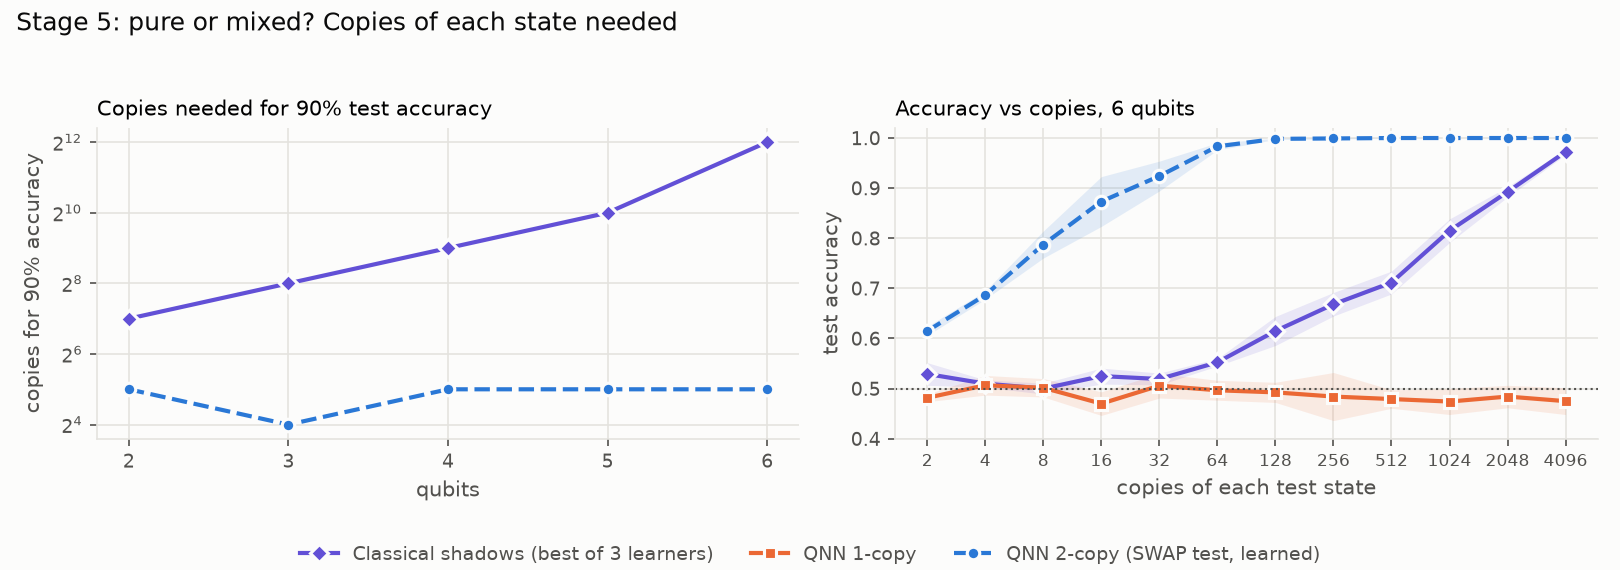
\includegraphics[width=\linewidth]{figures/entangle_purity.png}
\caption{Pure vs.\ mixed states, exact simulation. Left: copies needed for 90\% accuracy (mean curves). Right: accuracy vs.\ copies at 6 qubits (mean and spread over 3 seeds).}
\label{fig:purity}
\end{figure}

\paragraph{Hardware.} Only the entanglement (2 qubits) and Ising-phase (4 qubits) classifiers have been run on \texttt{ibm\_marrakesh}, on 10 test states each with 512 copies; at that size the runs are an end-to-end check. The purity test has not been run on hardware.

\section{Related work}
\textbf{Benchmarking.} Bowles et al.~\cite{bowles2024better} benchmark QML models at scale and find that classical baselines often match or beat them; our protocol follows the same spirit at small scale, adding hardware. \textbf{Encoding and expressivity.} Data re-uploading~\cite{perezsalinas2020reuploading} and the Fourier view of encoding~\cite{schuld2021encoding} explain why the encoding dominated our ablation. \textbf{Dequantization.} Quantum-inspired classical algorithms~\cite{tang2019dequantized} and random-Fourier-feature approximations of variational QML models~\cite{landman2022rff} suggest that circuits like ours may be classically approximable; we did not test such surrogates. \textbf{Learning from quantum data.} Exponential separations between learners with and without quantum memory are proven in~\cite{chen2021memory,aharonov2022qam} and demonstrated on hardware in~\cite{huang2022experiments}; our purity experiment is a small-scale, simulated illustration of that separation against one classical-shadow method~\cite{huang2020shadows}. \textbf{Trainability.} Barren plateaus~\cite{mcclean2018barren} and their dependence on the cost function~\cite{cerezo2021cost} match the training failure we observed. \textbf{Hardware characterisation.} Capability benchmarks~\cite{proctor2022capabilities} and error mitigation~\cite{temme2017mitigation} address device noise systematically; we used no mitigation and characterise only the output bias of one shallow circuit.

\section{Discussion and limitations}
In these experiments a quantum model showed an advantage only where it could hold two copies of a quantum state at once, which matches theory~\cite{huang2022experiments,chen2021memory}; we illustrate that result rather than extend it, and only against the classical methods we tested. On classical data the circuit classifies features chosen by a classical encoder, and tuned classical models on the same features do as well or slightly better.

Limitations: (i) all simulations use at most 8 qubits and are exact, so nothing here is classically hard; (ii) design choices were explored with test-set feedback (Section~\ref{sec:protocol}); (iii) the ablation uses one dataset; (iv) the hardware study uses one device, one circuit family, 200 inputs per task and few runs within two sessions, and the bias may drift with calibration; (v) prediction changes are tested under an independence assumption across inputs and runs; (vi) CVE severity from descriptions alone approximates CVSS scoring; (vii) the purity separation has not been tested on hardware.

\paragraph{Reproducibility.} Code, configurations, result files and job identifiers are in \url{https://github.com/H3XY/AGI} and \url{https://github.com/H3XY/Entangle}; Appendix~\ref{app:repro} lists versions, commands and jobs. During this work we found that \texttt{qiskit-ibm-runtime}~0.44.1 declares Qiskit~1.x support but fails to transpile for real devices on it; we reported it upstream (Qiskit/qiskit-ibm-runtime\#3563).

\paragraph{Acknowledgements.} Code, experiments and drafting were carried out with assistance from an AI coding assistant (Claude, Anthropic); an independent critical review was obtained from another AI model (ChatGPT, OpenAI). The author reviewed all results and takes responsibility for the content. We thank IBM Quantum for Open Plan access.

\bibliographystyle{unsrtnat}
\bibliography{refs}

\appendix
\section{Reproducibility details}\label{app:repro}
\sloppy
\textbf{Software.} Python 3.12.16; qiskit 1.4.6; qiskit-ibm-runtime 0.43.1 (0.44.x fails on Qiskit~1.x); qiskit-machine-learning 0.8.4; qiskit-aer 0.18.2; numpy 2.4.6; scikit-learn 1.9.1; sentence-transformers 6.2.0. Training uses Qiskit's exact reference \texttt{Sampler}.

\textbf{Commands} (AGI repository): \texttt{python train.py --task sentiment|cve}; \texttt{python -m benchmark.uncertainty} (Table~\ref{tab:text}); \texttt{python -m benchmark.ablation} (Table~\ref{tab:ablation}); \texttt{python -m benchmark.hardware\_study} and \texttt{benchmark.hardware\_study\_report} (Table~\ref{tab:hw}; \texttt{--fake-only} reproduces the noise-model rows without IBM access); \texttt{python -m ibmq.job\_log}. Result files are in \texttt{results/}.

\textbf{IBM jobs} (\texttt{ibm\_marrakesh}, Open Plan; times UTC). 200-input study, 9~November 2026: CVE \texttt{dbov06tt7fqc7388gab0}, \texttt{dbov3ttt7fqc7388gfrg}; sentiment \texttt{dbov4itt7fqc7388ggog}. Earlier 40-input runs, 8--9~November 2026: benchmark \texttt{dbolcblt7fqc73881hv0}, \texttt{dbold1tt7fqc73881iqg}, \texttt{dboldboou4as73cs9lcg}, \texttt{dbole58qtr0c738d1ccg}, \texttt{dbolhc0qtr0c738d1ihg}; CVE repeats \texttt{dbomf5gou4as73csbdmg}, \texttt{dbomfas4148s739t8q1g}, \texttt{dbomfg5t7fqc73883ctg}. The full list with timestamps and quantum seconds is in \texttt{results/ibm\_jobs.json}.

\textbf{Calibration} (physical qubits 0--3 at the start of the 200-input study): readout error 0.006--0.024; CZ error 0.0022--0.0027; full values per qubit, including $T_1$ and $T_2$, in \texttt{results/hardware\_study/*.json}.
\end{document}
